% article example for classicthesis.sty
\documentclass[10pt,a4paper]{article} % KOMA-Script article scrartcl
\usepackage{lipsum}     %lorem ipsum text
\usepackage{titlesec}   %Section settings
\usepackage{titling}    %Title settings
\usepackage[margin=10em]{geometry}  %Adjusting margins
\usepackage{setspace}
\usepackage{listings}
\usepackage{amsmath}    %Display equations options
\usepackage{amssymb}    %More symbols
\usepackage{xcolor}     %Color settings
\usepackage{pagecolor}
\usepackage{mdframed}
\usepackage[spanish]{babel}
\usepackage[utf8]{inputenc}
\usepackage{longtable}
\usepackage{multicol}
\usepackage{graphicx}
\graphicspath{ {./Images/} }
\setlength{\columnsep}{1cm}

% ====| color de la pagina y del fondo |==== %
\pagecolor{black}
\color{white}



\begin{document}
    %========================{TITLE}====================%
    \title{\rmfamily\normalfont\spacedallcaps{ Clase 5 graficar variables en espacios n dimensionales }}
    \author{\spacedlowsmallcaps{Rodrigo Castillo}}
    \date{\today} 
    
    \maketitle
     

     % ====| Loguito |==== %
    
\includegraphics[width=0.1\linewidth]{negro_cara.png}
    %=======================NOTES GOES HERE===================%
    \section{Ejemplo facil de entender}
        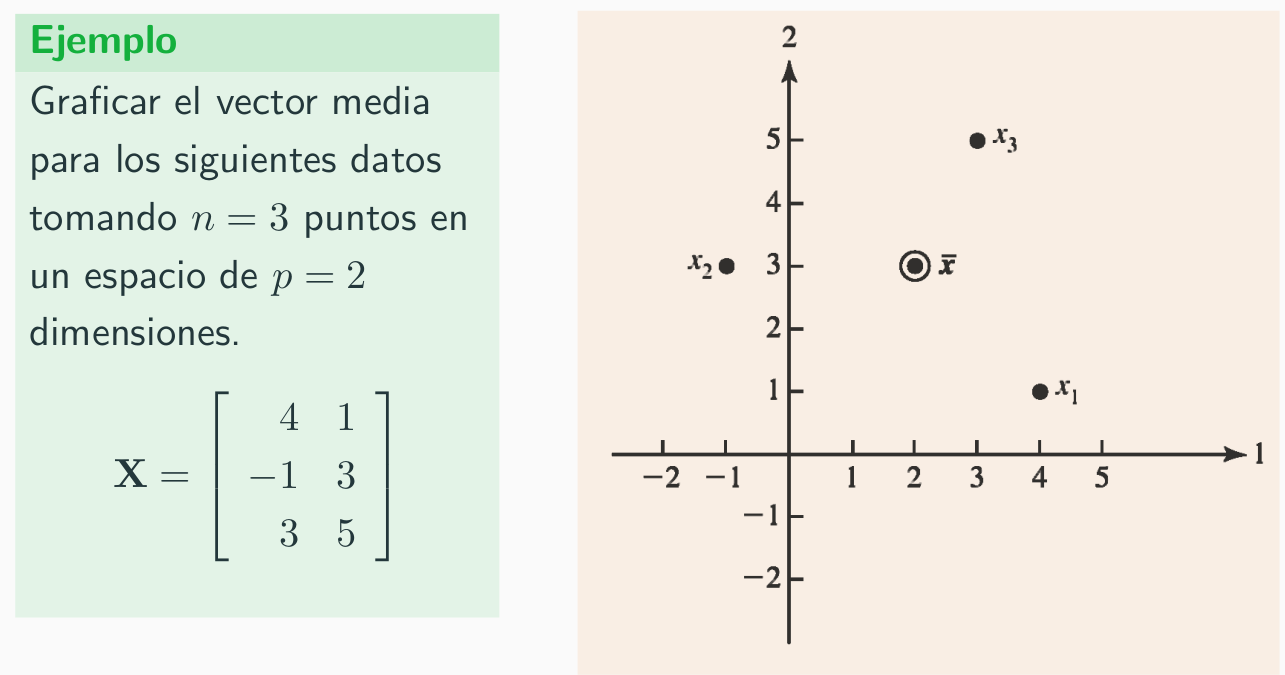
\includegraphics[width=0.8\linewidth]{ejemplofacil.png} 
        \\ el caso anterior se puede extender para N dimensiones 
    \section{graficar p vectores en n dimensiones}
        \subsection{primer ejemplo}
            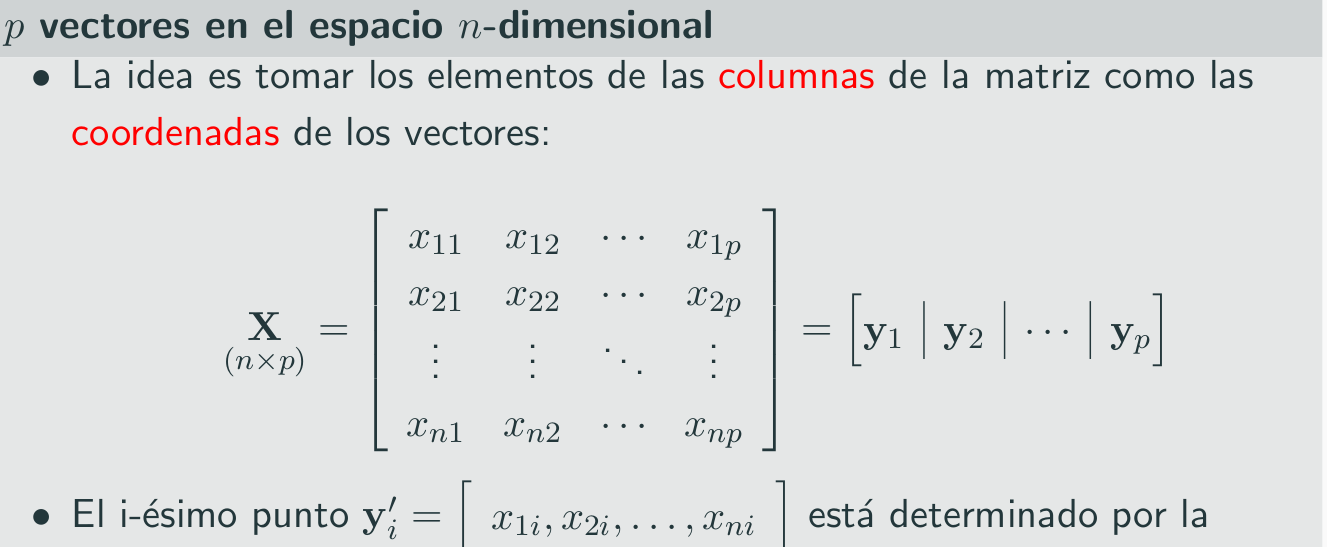
\includegraphics[width=0.8\linewidth]{pndimensional.png}
            \\ igual que el ejemplo anterior de todas formas
    \section{relacion entre la desviacion y la desviacion estandar}
        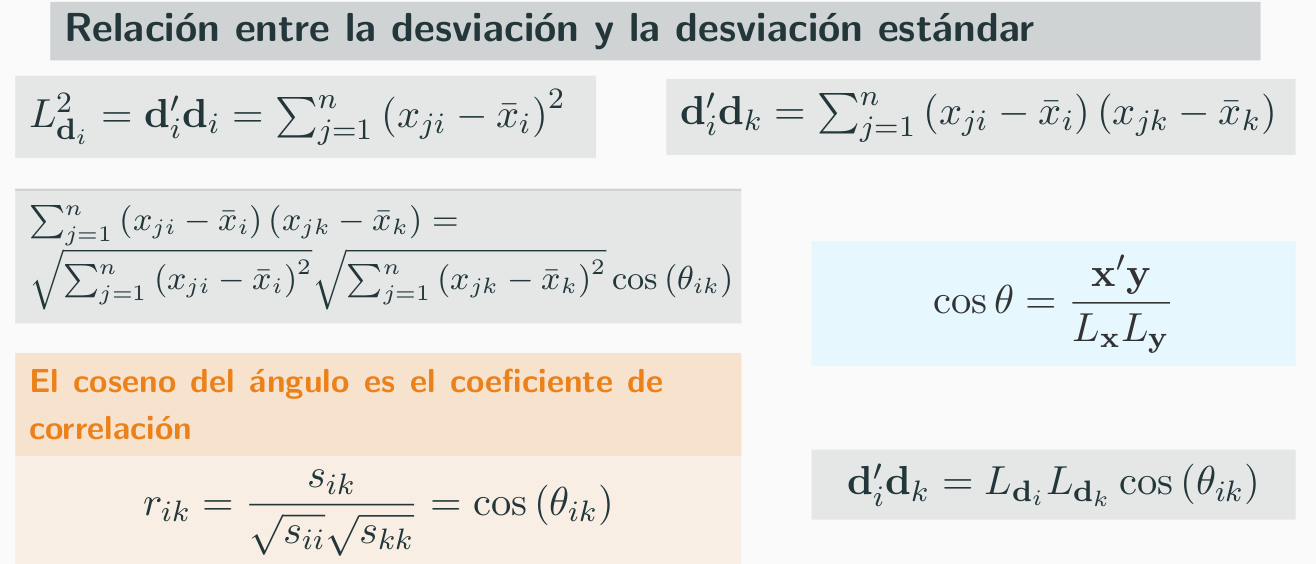
\includegraphics[width=0.8\linewidth]{relaciondesv.png}
        \\ 

    \section{media poblacional y varianza poblacional}
        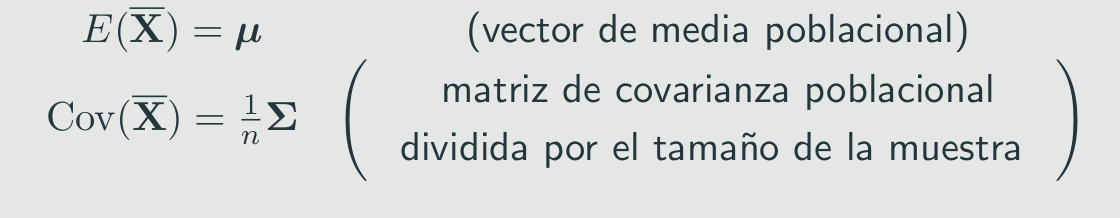
\includegraphics[width=0.8\linewidth]{media_pob.png}
        \\     
    \section{estimador para \sum_{  }^{ } }
        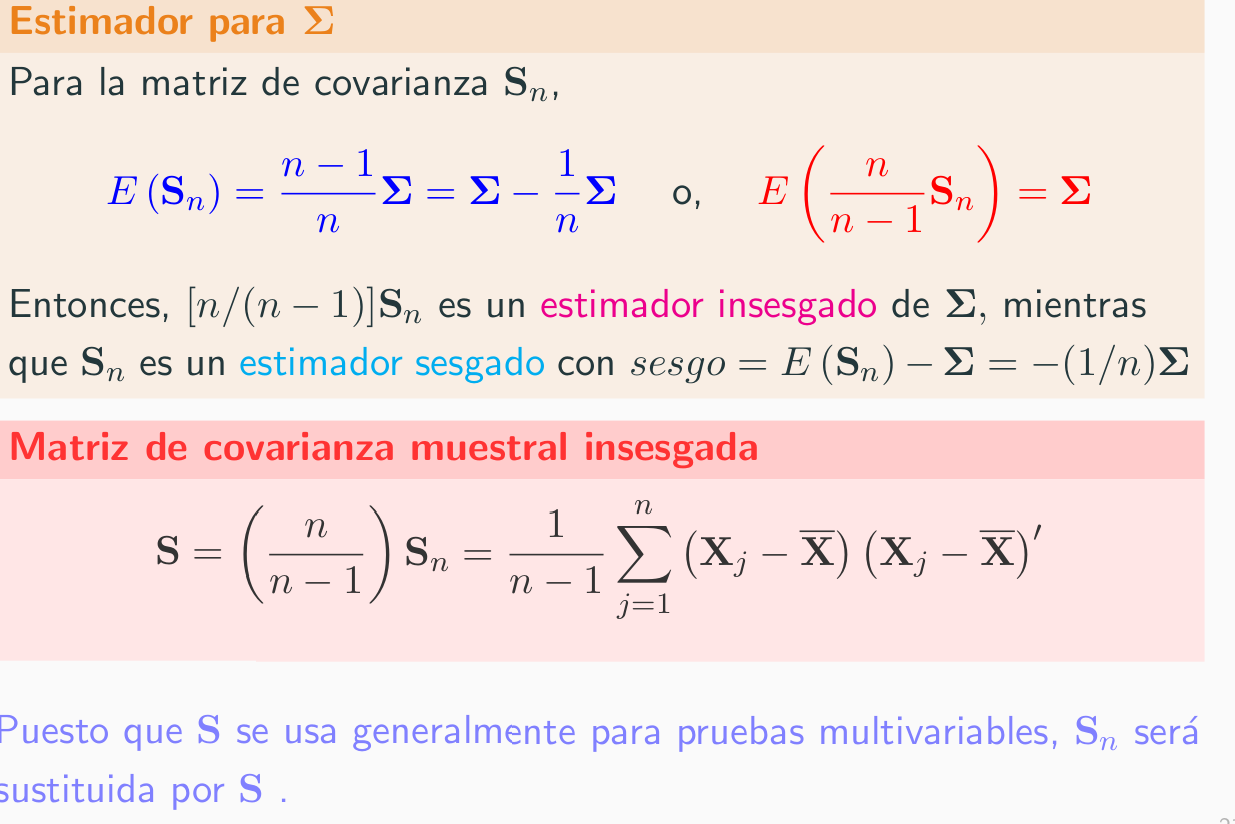
\includegraphics[width=0.8\linewidth]{estimador.png}
    \section{Preguntas}
        Preguntar bien como se calcula el estimador para $ \sum  $  y para que sirve







    %=======================NOTES ENDS HERE===================%
    
    % bib stuff
    \nocite{*}
    \addtocontents{toc}{\protect\vspace{\beforebibskip}}
    \addcontentsline{toc}{section}{\refname}    
    \bibliographystyle{plain}
    \bibliography{../Bibliography}
\end{document}
